\documentclass[11pt]{article}
\usepackage[utf8]{inputenc}
\usepackage[T1]{fontenc}
\usepackage{mathptmx}
\usepackage{microtype}
\usepackage[margin=1in]{geometry}
\usepackage{amsmath,amssymb}
\usepackage{graphicx}
\usepackage{booktabs}
\usepackage{caption}
\usepackage[round,authoryear]{natbib}
\usepackage{xcolor}
\usepackage[hidelinks]{hyperref}
\usepackage{newunicodechar}
\usepackage{setspace}
\usepackage{lineno}
\newunicodechar{−}{\ensuremath{-}}
\newunicodechar{×}{\ensuremath{\times}}
\newunicodechar{±}{\ensuremath{\pm}}
\newunicodechar{Δ}{\ensuremath{\Delta}}
\newunicodechar{†}{\ensuremath{\dagger}}
\captionsetup{font=small,labelfont=bf}
\bibliographystyle{plainnat}
\setcitestyle{authoryear,round,semicolon}
\providecommand{\tightlist}{\setlength{\itemsep}{0pt}\setlength{\parskip}{0pt}}
\onehalfspacing
\linenumbers

\title{The Bitter Lesson comes to genomic prediction: an untuned tabular foundation model matches or beats specialized methods}
\author{Lex Flagel\\[2pt]\small University of Minnesota, St.\ Paul, MN, USA}
\date{}

\begin{document}
\maketitle

\begin{abstract}
Genomic prediction (GP) is dominated by models designed around assumptions about how genetic variation affects phenotypes. We asked how well a general-purpose pretrained tabular foundation model does instead when given marker genotypes directly, with no genetics-specific modeling and no tuning. Using a published comparison of 18 GP methods on 18 traits in six plant species (327--5,014 lines, 4,234--244,781 markers), we benchmarked TabPFN-3.5. Against the published means, TabPFN-3.5 ranked first on 11 of 18 traits and had the best median rank. Because published results did not report their data splits, we reran GBLUP, RKHS and elastic-net models on the same splits as TabPFN-3.5. Against the best of these, TabPFN-3.5 was significantly behind on only one trait, spruce wood density (−0.032), and ahead on 12 of 18, with significant gains on all three soybean traits (+0.017 to +0.041 in correlation, 3--9\% relative), maize yield (+0.043) and rice flowering time (+0.047). In the soybean panel, which had by far the largest training set (4,011 lines), its advantage was clearest. When whole soybean families were held out, every model lost most of its accuracy and TabPFN-3.5 performed on par with GBLUP and RKHS, so its soybean advantage depends on the families represented in training. Consistent with Sutton's ``Bitter Lesson'', a general learner that gets its knowledge from pretraining rather than from the domain matches the accuracy of decades of specialized GP models without any adaptation, and exceeds it where data are most plentiful.
\end{abstract}

\section{Introduction}

Genomic prediction (GP), also called genomic selection, predicts an individual's breeding value or phenotype from genome-wide markers \citep{meuwissen2001}. A model is trained on individuals with both genotypes and phenotypes and then applied to individuals that have only been genotyped. Because genotyping is fast and cheap relative to phenotyping, GP lets breeders screen and select candidates before phenotypes exist. It has become routine in dairy cattle \citep{hayes2009,wiggans2017}, where it sharply shortened generation intervals for sires \citep{garciaruiz2016}, and in plant breeding programs across major crops \citep{heffner2009,crossa2017}. The USDA estimated that genomic selection returned about \$4 billion to the US dairy industry in its first nine years \citep{rexroad2019}.

Under the breeder's equation, the rate of genetic gain scales linearly with prediction accuracy \citep{falconer1996}. Gains of a few hundredths in correlation therefore compound across generations, which has motivated two decades of method development. The dominant methods are ridge-regression BLUP and its equivalent GBLUP \citep{vanraden2008,endelman2011}, and the ``Bayesian alphabet'' of marker-effect priors such as BayesA, BayesB and the Bayesian LASSO \citep{meuwissen2001,delosCampos2013,gianola2013}. Kernel methods such as RKHS regression capture some non-additive signal \citep{gianola2006}, and explicit epistatic kernels have also been proposed \citep{jiang2015}.

Machine learning, and deep learning in particular, has been tested extensively for GP, with mixed results. Large comparisons generally find that neural networks do not consistently beat linear models and are sensitive to tuning \citep{bellot2018,perezenciso2019,montesinos2021}. The six-species benchmark of \citet{azodi2019} compared 18 methods and found that no single method was best and neural networks never ranked first. A recent ten-species benchmark found tuned gradient-boosting and random-forest models only marginally more accurate than Bayesian regressions, by about 0.01--0.03 in correlation \citep{quesadatraver2025}. Flexible models thus give small and inconsistent gains. This may reflect the structure of GP datasets, in which hundreds to a few thousand individuals share tens of thousands of correlated markers, while genetic variance is predominantly additive \citep{hill2008}, limiting the benefits of model flexibility when each model is trained on a single, relatively small dataset.

Formally, a GP dataset is an $N \times M$ matrix of marker genotypes ($N$ individuals, $M$ markers), an $N \times P$ matrix of phenotypes, and sometimes covariates. Framed this way, GP is a standard supervised regression problem where we learn a mapping from a row of genotypes to a phenotype on individuals that have both, then apply it to individuals that have only genotypes. Most GP methods do not treat it so generically. They are built around assumptions about how genetic variation produces phenotypes, such as relationship matrices, priors on the distribution of marker effects, and kernels encoding additive or epistatic covariance. Designing such models is a central activity of the field, and much of its literature consists of new priors, kernels or architectures, each tuned to the structure of genetic data.

Sutton's ``Bitter Lesson'' \citep{sutton2019} argues that, across AI research, general methods that leverage computation have repeatedly overtaken methods built on human knowledge of the domain. GP has invested heavily in hand-designed priors, kernels and architectures, whose gains over one another are typically small and dataset-specific \citep{azodi2019,quesadatraver2025}. The Bitter Lesson predicts that larger gains will come instead from general learners that convert computation into accuracy. In GP, the data per problem often remains small, so the computation has to be spent elsewhere. TabPFN shifts that computation to pretraining on millions of synthetic supervised-learning datasets, allowing it to learn general patterns of prediction that transfer to new problems without redesigning the model for each one.

TabPFN is a transformer designed to approximate Bayesian posterior prediction. At inference, it takes the training rows and their labels as context and predicts new rows in a single forward pass, without gradient updates or hyperparameter search \citep{muller2022,hollmann2023,hollmann2025}. It has been strongest when $N$ is in the hundreds to low thousands, which is exactly the training-set size of many GP datasets. Until recently, however, its feature limits were far below $M$ for a typical marker panel. Earlier TabPFN applications to high-dimensional biological data therefore compressed or pre-selected features. As a recent example, in wheat, TabPFN served as one learner in an ensemble trained on about 8,300 SNPs selected with GWAS, a meta-QTL database and model-based feature importance \citep{ren2025}. The TabPFN-3 and TabPFN-3.5 releases raised the number of features that can be supplied to the model, and TabPFN-3.5 accepts up to 20,000 columns, the limit used in this study \citep{priorlabs2026a,priorlabs2026b,priorlabs2026c}. With these expanded feature limits, TabPFN can be applied more directly to marker panels and may capture nonlinear gene interactions when they contribute to genetic variation, without requiring their form to be specified in advance, as epistatic kernels do \citep{jiang2015}.

Here we take the Bitter Lesson approach to GP. We give TabPFN-3.5 the marker matrix directly, with no genetics-specific modeling, no trait-based marker selection and no tuning, and ask how close a general-purpose pretrained model comes to methods built for the problem. We benchmark it on the 18 species-trait combinations of \citet{azodi2019} and compare it with the 18 published methods. Because published results do not give their random training splits, we also rerun GBLUP, RKHS and elastic-net models on identical splits to those given TabPFN-3.5. For the four species whose $M$ exceeds TabPFN's limit, we test a simple input of principal components plus evenly thinned markers. Because TabPFN then sees a reduced input while the other models see every marker, we also fit GBLUP and an elastic net to the same reduced input, to separate the effect of the input from the effect of the model. Finally, we test whether TabPFN's advantage holds when entire soybean families are held out, a harder and more breeding-relevant validation. Among all 19 methods, TabPFN-3.5 was the most accurate on 11 of 18 tests and had the best median rank. On identical splits, it was significantly behind the best rerun model on only one test (spruce wood density) and ahead on 12 of 18, with significant gains on five: all three soybean traits, maize yield and rice flowering time. When whole soybean families were held out, however, TabPFN-3.5 lost its advantage and performed on par with GBLUP and RKHS.

\section{Materials and methods}

\subsection{Data}

We used the genotype, phenotype and fold-assignment files (100 random partitions of the lines into five folds) of \citet{azodi2019}, deposited on Dryad under CC0 (doi:10.5061/dryad.xksn02vb9). The original studies that produced each dataset are cited in Table~\ref{tab:data}. Markers are coded −1/0/1; the rice data also include a small fraction (about 3\%) of imputed, non-integer dosages. Each species has three traits. The datasets span a 15-fold range in training-set size and a 58-fold range in marker number.

\begin{table}[tbp]
\centering
\caption{Datasets, from \citet{azodi2019}. Each species has three traits.}
\label{tab:data}
\footnotesize
\setlength{\tabcolsep}{4pt}
\begin{tabular}{@{}p{1.9cm}p{3.0cm}rrp{3.0cm}p{3.6cm}@{}}
\toprule
Species & Population & Lines & Markers & Traits & Original data \\
\midrule
Soybean & SoyNAM RILs & 5,014 & 4,234 & height, R8, yield & \citet{xavier2016} \\
White spruce & tree breeding population & 1,722 & 6,930 & DBH, height, wood density & SmartForests project; SNP chip from \citet{beaulieu2014} \\
Rice & IRRI elite breeding lines & 327 & 57,542 & flowering time, height, yield & \citet{spindel2015} \\
Sorghum & diversity panel (NPGS) & 451 & 56,299 & grain moisture, height, yield & \citet{fernandes2018} \\
Switchgrass & N.\ Switchgrass Association Panel & 514 & 217,150 & anthesis date, height, standability & \citet{lipka2014,evans2015,evans2018} \\
Maize & diversity panel & 391 & 244,781 & flowering time, height, yield & \citet{hansey2011,hirsch2014} \\
\bottomrule
\end{tabular}
\end{table}

\subsection{Validation design}

For each trait we used 10 replicate 80/20 holdouts, which matches the design of \citet{azodi2019}. Because their exact test sets were not published, our splits are different random draws from the same fold files. Accuracy is the Pearson correlation between predicted and observed phenotypes in the held-out lines, averaged over replicates. No information from test lines enters model fitting, except that the genomic relationship matrices of the kernel models are computed from the markers of all lines, as in the rrBLUP script of \citet{azodi2019} (code at \url{https://github.com/ShiuLab/Manuscript_Code}).

To test generalization across families, we also built a leave-families-out design for soybean. In each of 10 replicates, 8 of the 38 SoyNAM families (21\% of lines on average; 1,031--1,096 lines) were held out at random, and models were trained on the other 30 families.

\subsection{TabPFN}

We used \texttt{TabPFNRegressor} from the \texttt{tabpfn} Python package (version 9.1.0) with the TabPFN-3.5 weights \citep{priorlabs2026b}, default settings, no hyperparameter tuning, and \texttt{random\_state} set to the replicate number. TabPFN does not make a single prediction per test line. Much as a random forest averages its trees, TabPFN averages several forward passes of the model, called ensemble members, each run on a slightly different view of the training data. In the tabpfn 9.1.0 package, each member sees at most 768 input columns. The default of 8 members can therefore include at most $8 \times 768 = 6{,}144$ columns between them, and with a wider input some markers would never be seen by any member. For such inputs we raised the number of members to the smallest value that covers every column at least once: $\lceil M/768 \rceil$ members for $M$ input columns, which is 10 for the 6,930 spruce markers. Soybean's 4,234 markers fit within the default 8 members. Apart from the number of members, all settings were left at their defaults. The open TabPFN-3.5 weights are licensed for non-commercial use; commercial use requires a separate license agreement with Prior Labs.

\emph{Raw markers (soybean, spruce).} All 4,234 and 6,930 markers were supplied as-is.

\emph{Hybrid input (rice, sorghum, maize, switchgrass).} These have 56,000--245,000 markers, more than the 20,000 columns TabPFN-3.5 accepts \citep{priorlabs2026c}. For each replicate we supplied (1) the top 100 principal components of all markers, computed on the training lines only with test lines projected onto them, and (2) 19,900 raw markers chosen at evenly spaced ranks after sorting by chromosome and position. We used the TabPFN-3.5 package's \texttt{constant\_and\_balanced} feature subsampling so that the 100 components are given to every ensemble member and the thinned markers are divided among members. Each member therefore sees all 100 components plus 668 of the markers, and 30 members are needed to include all 19,900 markers.

\emph{Alternative inputs.} We also ran principal components alone (all species), thinned markers alone (four large species) and, for rice, all 57,542 markers with the package's pretraining limits disabled (\texttt{ignore\_\allowbreak{}pretraining\_\allowbreak{}limits}).

\subsection{Comparison models}

All comparison models were fit on exactly the same training and test lines as TabPFN.

\begin{itemize}
\tightlist
\item
  \textbf{GBLUP.} $y = \mu + g + e$ with $g \sim N(0, \sigma^2_g K)$, fit by REML on the training lines; predictions are the BLUPs of $g$ for test lines. K was built as in the rrBLUP script of Azodi et al.: $K = ZZ' / \overline{\mathrm{diag}(ZZ')}$, with $Z$ the column-standardized marker matrix of all lines. Our Python implementation reproduces \texttt{rrBLUP::kin.blup} \citep{endelman2011} to within $10^{-6}$ in correlation on every soybean and spruce replicate.
\item
  \textbf{RKHS.} The same REML model with a Gaussian kernel $K_{ij} = \exp(-d^2_{ij} / h)$, where $d^2_{ij}$ is the mean squared difference between standardized marker profiles and $h$ is its median over pairs \citep{gianola2006,delosCampos2013}.
\item
  \textbf{Elastic net (ENet).} Penalized regression with an L1/L2 mixing ratio of 0.5 and the penalty chosen from 30 values by 5-fold cross-validation within the training lines (scikit-learn \texttt{ElasticNetCV}; \citealp{pedregosa2011}). We call it ENet to distinguish it from the EN5 and EN11 ensembles of \citet{azodi2019}. ENet used all markers for soybean and spruce. For the four large species it was fit only on the hybrid input (below): on 56,000--245,000 markers each fit takes minutes, and GBLUP already covers the all-marker linear model.
\item
  \textbf{Comparison models on the hybrid input.} For the four large species, GBLUP with K built only from the 19,900 thinned markers (GBLUP-thin) and an elastic net on the same 100 PCs + 19,900 markers that TabPFN received (ENet-hybrid). On these species TabPFN and the other models differ in both the model and the input (TabPFN sees PCs plus thinned markers, the other models see every marker). Giving the other models TabPFN's reduced input removes the second difference.
\end{itemize}

\subsection{Comparison with published results}

Table S5 of \citet{azodi2019} gives the mean accuracy of 18 methods for each species and trait: rrBLUP, Bayesian ridge regression, BayesA, BayesB, Bayesian LASSO, three support vector regressions, random forest, gradient tree boosting, five neural network variants, a convolutional network, and two ensembles (EN5, EN11) that average 5 or 11 of these methods. We ranked TabPFN's mean accuracy among these 18 published means. Because published and TabPFN means come from different splits, this ranking is descriptive; the comparison models rerun on identical splits carry the formal comparisons.

\subsection{Statistics}

For each species and trait we computed the per-replicate difference in accuracy between TabPFN and each comparison model. Within each replicate the training and test lines are disjoint, but across replicates both training sets and test sets overlap (any two test sets share about 20\% of their lines), so a naive paired t-test, which treats replicates as independent, understates the variance. We therefore report the mean difference with a 95\% interval from the corrected resampled t-test of Nadeau and Bengio (2003), using a test-to-training size ratio of 20/80 = 0.25, along with the number of replicates in which TabPFN was more accurate.

\subsection{Software and compute}

TabPFN ran on the integrated GPU of an Apple M4 Pro chip. Comparison models ran on the CPU of the same chip, in Python 3.13 with NumPy, SciPy and scikit-learn 1.9.1. Run times are reported per fit.

\section{Results}

\subsection{Against published methods, TabPFN-3.5 has the best median rank}

With no tuning, and among 19 methods (itself plus the 18 published), TabPFN-3.5 had the highest mean accuracy on 11 of 18 species-trait tests and was in the top three on one more. The next best method, the EN11 ensemble of 11 methods from \citet{azodi2019}, had a median rank of 3.5; TabPFN-3.5's median rank was 1 (Table~\ref{tab:ranks}).

\begin{table}[tbp]
\centering
\caption{Rank of TabPFN-3.5 among the 18 published methods of \citet{azodi2019} (Table S5 of that paper), over the 18 species-trait tests. Only the seven methods with the best median ranks are shown.}
\label{tab:ranks}
\small
\begin{tabular}{lrrr}
\toprule
Method & Median rank (of 19) & Tests ranked first & Tests in top 3 \\
\midrule
TabPFN-3.5 & 1 & 11 & 12 \\
EN11 (ensemble of 11 methods) & 3.5 & 2 & 9 \\
BayesA & 5 & 0 & 7 \\
EN5 (ensemble of 5 methods) & 5.5 & 0 & 4 \\
Bayesian ridge regression & 6 & 2 & 2 \\
rrBLUP & 6 & 0 & 6 \\
BayesB & 7 & 2 & 2 \\
\bottomrule
\end{tabular}

\end{table}

On the six tests where it saw every marker (soybean, spruce), TabPFN ranked first every time; on the hybrid input (rice, sorghum, maize, switchgrass), it ranked first on 5 of 12. Its weakest species was sorghum, where it ranked 8th to 13th. Per-test accuracies for every model are in Table~S1.

These ranks compare TabPFN with published means from different random splits, and that difference matters. On the five species other than rice, our GBLUP was within about 0.04 of the published rrBLUP on every trait. On rice it was far higher: 0.186 higher for yield, 0.140 higher for flowering time, and 0.05 higher for height. The published rice rrBLUP appears anomalous. In Azodi et al.'s own results, rrBLUP and Bayesian ridge regression, which fit nearly the same model, agree within 0.02 on all 15 non-rice tests but differ by 0.04--0.12 on rice. Against their Bayesian ridge regression, our GBLUP agrees more closely for rice flowering time (0.557 vs 0.539) and height (0.396 vs 0.385) but remains higher for yield (0.458 vs 0.363), a gap we cannot explain. As a check, our own GBLUP, rerun on our splits, also ranked first on 5 of 18 tests against the published table, so part of TabPFN's lead in this ranking reflects the splits rather than the model. The comparisons on identical splits below are the main evidence.

\subsection{On identical splits, TabPFN matches or beats strong comparison models, with clear wins in soybean}

Compared with the best of GBLUP, RKHS and GBLUP-thin on the same splits, TabPFN's mean accuracy was higher on 12 of 18 tests (Figure~\ref{fig:paired}). The corrected interval excluded zero on six: on spruce wood density TabPFN was worse (−0.032), and on all three soybean traits (+0.017 to +0.041), maize yield (+0.043) and rice flowering time (+0.047) it was better. The other 12 differences were within split-to-split noise.

\begin{figure}[tbp]
\centering
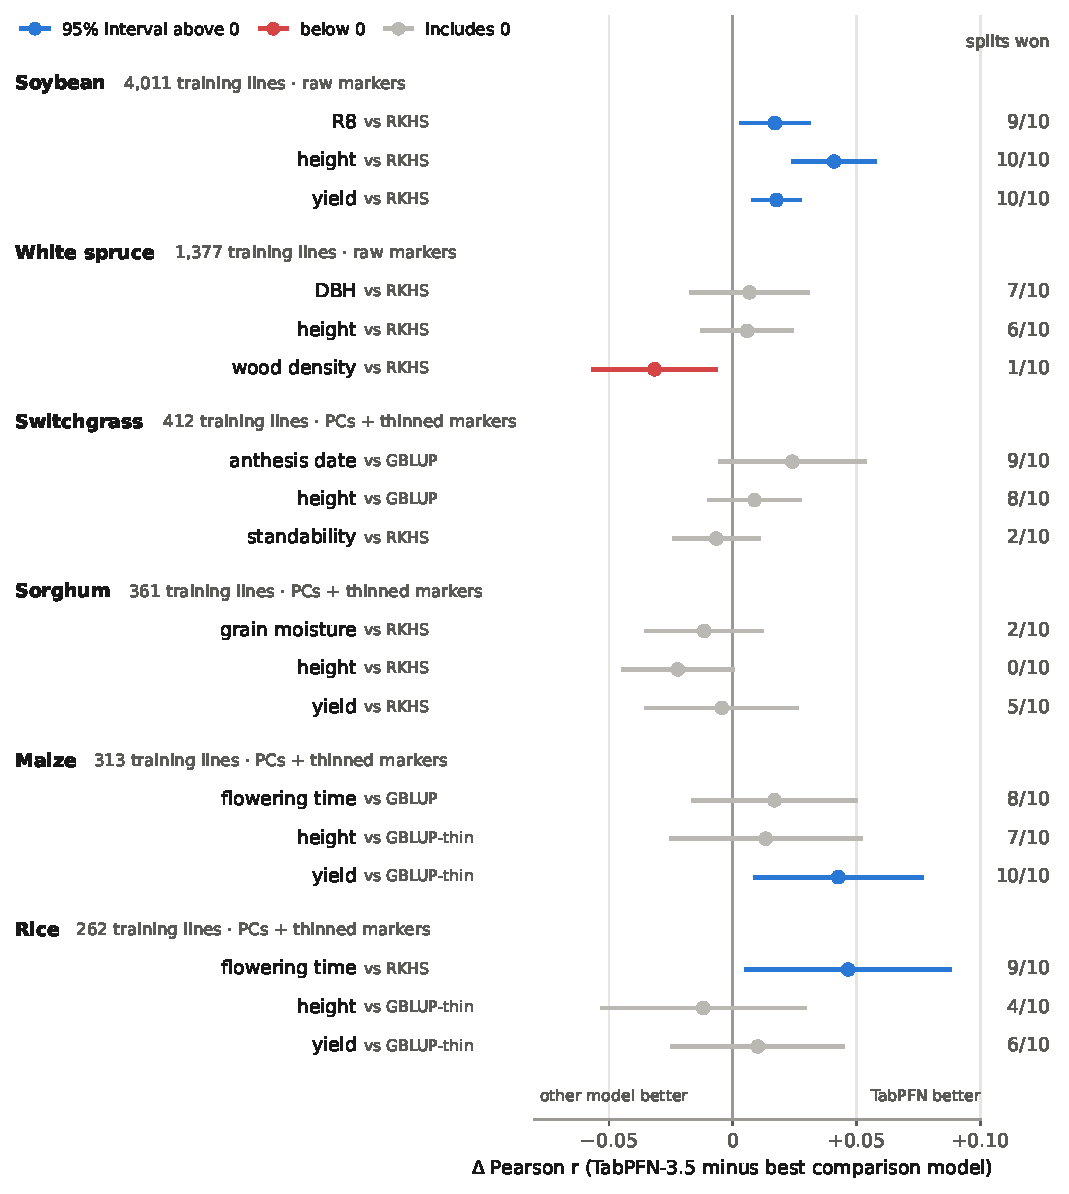
\includegraphics[width=\linewidth]{figures/figure1.pdf}
\caption{\textbf{TabPFN-3.5 matches or beats the comparison models on identical splits, with clear gains in soybean.} Each point is the mean difference in Pearson r between TabPFN-3.5 and the most accurate of GBLUP, RKHS and GBLUP-thin for that test, over the same 10 replicate 80/20 splits; horizontal bars are 95\% intervals from the corrected resampled t-test \citep{nadeau2003}. Blue: interval above zero; red: below zero; grey: includes zero. TabPFN was ahead on 12 of 18 tests, with intervals above zero on 5 and below zero on 1. The right-hand column gives the number of splits on which TabPFN was more accurate. Species are ordered by training-set size, and the label beside each gives TabPFN's input: all raw markers, or 100 principal components plus 19,900 thinned markers.}
\label{fig:paired}
\end{figure}

With the largest training set (4,011 lines), soybean is the one species where TabPFN won every trait, on 9 or 10 of 10 splits each time. Its intervals there are also the tightest (±0.010 to ±0.017), because its 1,003-line test sets measure accuracy precisely. The comparison is also conservative for TabPFN because of the winner's curse phenomenon. For each test, TabPFN is compared with whichever of the three comparison models scored highest on these same splits, and that best score tends to overstate the chosen model's true accuracy, so the differences in Figure~\ref{fig:paired} are, if anything, understated.

Of the comparison models, RKHS was strongest on 11 of 18 tests. It was not among the methods of \citet{azodi2019}, yet on spruce it matched or beat every published method. ENet was never the strongest comparison model. On the large species it was fit to the hybrid input (next section), and on soybean and spruce it trailed GBLUP by 0.01 to 0.20 (largest for soybean height, 0.264 vs 0.467) and TabPFN on every trait.

\subsection{The hybrid input works, and reducing markers costs the other models almost nothing}

For the four species with more markers than TabPFN accepts, combining 100 principal components with 19,900 thinned markers was better than either alone (Table~\ref{tab:inputs}). Across the 120 species-by-trait-by-split comparisons, the hybrid input beat thinned markers alone on 97 and principal components alone on 82.

The 20,000-feature limit is not absolute. By default the package refuses wider inputs, but setting its \texttt{ignore\_\allowbreak{}pretraining\_\allowbreak{}limits} option lets it run on them, with a warning that the input lies outside the range the model was pretrained on and that accuracy may suffer. We tested this with all 57,542 rice markers. It gained nothing over thinned markers (0.486 vs 0.489; better on 10 of 30 trait-by-split comparisons) and took nearly three times as long per fit, so thinning was the better choice here, but the \texttt{ignore\_\allowbreak{}pretraining\_\allowbreak{}limits} option is open for panels where thinning might discard more information.

\begin{table}[tbp]
\centering
\caption{Mean accuracy (Pearson $r$) averaged over the three traits and 10 splits, by input, for the four species with more markers than TabPFN-3.5 accepts. *In 7 of 30 rice fits the elastic net kept no markers and predicted a constant, so the correlation is undefined; those fits are counted as $r = 0$.}
\label{tab:inputs}
\small
\setlength{\tabcolsep}{4pt}
\resizebox{\linewidth}{!}{\begin{tabular}{lrrrrrrr}
\toprule
Species & Markers & TabPFN: PCs & TabPFN: thinned & TabPFN: hybrid & GBLUP: all & GBLUP: thinned & ENet: hybrid \\
\midrule
Rice & 57,542 & 0.450 & 0.489 & 0.490 & 0.471 & 0.470 & 0.228* \\
Sorghum & 56,299 & 0.505 & 0.489 & 0.508 & 0.516 & 0.512 & 0.468 \\
Switchgrass & 217,150 & 0.727 & 0.711 & 0.734 & 0.725 & 0.720 & 0.687 \\
Maize & 244,781 & 0.602 & 0.586 & 0.609 & 0.583 & 0.583 & 0.556 \\
\bottomrule
\end{tabular}
}
\end{table}

Two checks address whether the reduced input, rather than the model, explains TabPFN's results. First, thinning to 19,900 markers changed GBLUP's mean accuracy by at most 0.005 per species, presumably because neighboring markers in these panels carry largely redundant information, so the comparison models in Figure~\ref{fig:paired} lose essentially nothing from the reduction. Second, given exactly TabPFN's hybrid input, an elastic net was less accurate than TabPFN on 107 of the 120 species-by-trait-by-split comparisons and fell behind it on every species, by 0.04 to 0.26 on average. The representation alone therefore does not explain TabPFN's accuracy.

How the markers are presented matters to TabPFN in a way it does not to GBLUP. For the four small panels, principal components alone came within 0.04 of the hybrid. For soybean, TabPFN on all 3,989 principal components, a lossless rotation of the markers, reached a mean of only 0.301, against 0.564 on the raw markers; for spruce the two were closer (0.339 vs 0.345). A ridge-type model is unchanged by such a rotation, so the soybean gap reflects how TabPFN uses its inputs; it appears to exploit the raw marker coding, which a rotation spreads across every component.

\subsection{On held-out soybean families, TabPFN performs on par with GBLUP and RKHS}

Random splits put sibling lines in both training and test sets, which inflates accuracy in structured populations \citep{habier2007,werner2020}. When whole SoyNAM families were held out, accuracy fell sharply for every model, TabPFN included (Table~\ref{tab:families}).

\begin{table}[tbp]
\centering
\caption{Soybean accuracy (Pearson $r$) with whole SoyNAM families held out, with GBLUP on random splits for reference. *In 5 of 10 height fits and 1 of 10 R8 fits, the elastic net kept no markers and predicted a constant, so the correlation is undefined; those fits are counted as $r = 0$.}
\label{tab:families}
\small
\begin{tabular}{lrrrrr}
\toprule
Trait & GBLUP, random & GBLUP, families & RKHS, families & ENet, families & TabPFN, families \\
\midrule
Height & 0.467 & 0.139 & 0.135 & 0.042* & 0.099 \\
R8 & 0.480 & 0.066 & 0.063 & 0.083* & 0.072 \\
Yield & 0.655 & 0.352 & 0.365 & 0.335 & 0.382 \\
\bottomrule
\end{tabular}

\end{table}

Across replicates and models, held-out-family accuracy ranged from below zero to 0.29 for height and R8, and from 0.10 to 0.59 for yield. Paired with GBLUP on the same held-out families, TabPFN's differences were −0.039 for height, +0.006 for R8 and +0.030 for yield, none distinguishable from zero, and it was more accurate on 15 of 30 splits (16 of 30 against RKHS).

These results suggest that TabPFN's advantage depends on the genetic backgrounds represented in the training population. When entire SoyNAM families were held out, its advantage over GBLUP and RKHS disappeared. This pattern does not indicate a limitation unique to foundation models like TabPFN. Rather, it highlights a broader challenge for genomic prediction when relationships between training and test individuals are reduced. TabPFN can compete with and beat specialized methods when predicting within the sampled population, but in soybean these results provide no evidence that it generalizes better to families absent from training.

\subsection{Run time}

Each TabPFN fit took 22--93 s on the integrated GPU of an Apple M4 Pro, against a few seconds or less for GBLUP and RKHS and 16--60 s for ENet on CPU. TabPFN needs no tuning, while many of the published methods required grid searches with repeated cross-validation \citep{azodi2019}. Even on a modest integrated laptop GPU, TabPFN genomic prediction runs take seconds or a few minutes, which is not appreciably slower than other CPU-based methods.

\section{Discussion}

Given only the marker matrix and no tuning, TabPFN was ahead of the strongest GP model on 12 of 18 published tests and significantly behind on just one. It was clearly worse only on spruce wood density, and clearly better on all three soybean traits, maize yield and rice flowering time. When the test lines came from soybean families absent from training, it performed on par with GBLUP and RKHS.

The gains are modest in absolute terms: +0.017 to +0.041 in correlation on soybean, or 3--9\% relative to the best comparison model. They are of the same size as the differences that separate established GP methods from one another \citep{azodi2019,quesadatraver2025}, and they came with no model design or hyperparameter search.

\subsection{Where TabPFN wins}

TabPFN's advantage was clearest in the dataset with the most training lines. Soybean also has the largest test sets, so its differences are measured most precisely, and with only 262--412 training lines in the four small panels (rice, maize, sorghum and switchgrass) a real advantage of 0.02 would often go undetected. Training-set size is confounded here with population type, however, because soybean is a set of related biparental families while the small panels are diverse collections. The family hold-out points to population structure: TabPFN's soybean advantage disappeared when the test families were absent from training, so it may also reflects better prediction among relatives within families rather than an advantage that grows with training-set size alone.

These experiments do not resolve why TabPFN beats GBLUP and RKHS on soybean. One possibility is non-additive genetic variance, which TabPFN can model without a specified form. Another is that its learned prior adapts shrinkage to the trait in a way a single-kernel model cannot. That TabPFN beat RKHS, which also captures some non-additive covariance, slightly favors the second, but simulations with known genetic architectures would be needed to tell them apart. Whichever it is, the family hold-out shows it applies to relatives already represented in training, such as haplotypes segregating within the same biparental families, rather than to marker effects that transfer across genetic backgrounds. The large loss on soybean when markers were replaced by principal components also shows that, unlike rotation-invariant linear models, TabPFN depends on the raw marker coding.

These results define where TabPFN's advantage applies. It appeared when test lines had full-sibs in the training set and was gone when whole families were held out, even though every SoyNAM family shares a common parent, so the held-out lines still had half-sib relatives in training. In our data, then, the advantage requires full-sib relatives of the candidates in training; whether a smaller advantage persists for more distant relatives could not be resolved here.

Full-sib relatives in the training set are routine in breeding. In plant breeding, sparse testing and early-generation selection phenotype part of each cross and predict the rest, as in biparental, recombinant inbred and doubled-haploid families of maize, wheat, barley and soybean. In animal breeding, pigs, poultry and especially aquaculture species such as salmon, tilapia and shrimp are bred in large full-sib families, and traits such as disease resistance are routinely measured on sibs of the selection candidates. Many forest tree programs likewise test full-sib families from controlled crosses. The open question is forward prediction: whether TabPFN helps when a model trained on one breeding cycle predicts new crosses in the next. These datasets lack the multi-cycle structure to test that, and it is the most important next validation.

\subsection{A test of the Bitter Lesson in genomic prediction}

Our results are consistent with the Bitter Lesson in GP. TabPFN, a model whose only knowledge comes from pretraining on synthetic data and scaled up with computation, reached the accuracy of methods refined over two decades for this problem, and exceeded it on random splits where data were most plentiful. The test is not entirely pure. For the four large panels, the feature limit forced us to reduce the marker input which imports some human design and taste in choosing principal components plus even marker thinning. That said, the knowledge involved is fairly generic. Principal component analysis is a general-purpose data-reduction method, and thinning relies only on marker order and the expectation that nearby markers are correlated through linkage. Both make much weaker assumptions about how genotype maps to phenotype than do relationship matrices, marker-effect priors and kernels of other GP methods. Furthermore, future TabPFN releases that accept more features would allow full marker panels for more of these datasets, removing even this step, and these comparisons are worth repeating when they arrive.

\section*{Use of generative AI}

Claude (Anthropic) was used extensively in this work: to write and run analysis code for the comparison models, to verify citations, and to draft and revise the manuscript text. ChatGPT (OpenAI) was used to review a draft. The author designed the study, ran the TabPFN analyses, checked all results, edited the text, and takes full responsibility for the content.

\section*{Data and code availability}

All data are from \citet{azodi2019}, deposited on Dryad under CC0 (\href{https://doi.org/10.5061/dryad.xksn02vb9}{doi:10.5061/dryad.xksn02vb9}); a checksum-verified mirror is included in the code repository. Code, per-replicate results for every model, and scripts to regenerate all tables and figures are at \href{https://github.com/flag0010/tabular-genomic-prediction-manuscript}{github.com/flag0010/tabular-genomic-prediction-manuscript} (Apache-2.0). The TabPFN-3.5 weights are licensed separately by Prior Labs under a non-commercial license.

\bibliography{references}

\clearpage
\appendix
\renewcommand{\thetable}{S\arabic{table}}
\setcounter{table}{0}
\section*{Supplementary material}

\begin{table}[htbp]
\centering
\caption{Mean accuracy (Pearson $r$) of every model on each species-trait test. TabPFN-3.5 and the comparison models are means over the same 10 replicate 80/20 splits. TabPFN-3.5 received raw markers for soybean and spruce and the hybrid input (100 PCs + 19,900 thinned markers) for the other four species. GBLUP-thin was run only where thinning was needed. ENet used all markers for soybean and spruce; $^\dagger$ marks ENet fit on the hybrid input. Fits where ENet kept no markers are counted as $r = 0$. Best published values are from Table S5 of \citet{azodi2019}, computed on different random splits; the last column ranks TabPFN-3.5 among those 18 published means.}
\label{tab:s1}
\footnotesize
\setlength{\tabcolsep}{3.5pt}
\resizebox{\linewidth}{!}{\begin{tabular}{llrrrrrlr}
\toprule
Species & Trait & TabPFN-3.5 & GBLUP & RKHS & GBLUP-thin & ENet & Best published & Rank of 19 \\
\midrule
Soybean & R8 & 0.505 & 0.480 & 0.488 & -- & 0.397 & 0.492 (EN11) & 1 \\
Soybean & height & 0.511 & 0.467 & 0.470 & -- & 0.264 & 0.468 (BayesA) & 1 \\
Soybean & yield & 0.677 & 0.655 & 0.660 & -- & 0.644 & 0.650 (EN11) & 1 \\
White spruce & DBH & 0.279 & 0.253 & 0.272 & -- & 0.185 & 0.275 (RF) & 1 \\
White spruce & height & 0.350 & 0.328 & 0.344 & -- & 0.268 & 0.346 (RF) & 1 \\
White spruce & wood density & 0.405 & 0.429 & 0.437 & -- & 0.395 & 0.398 (EN11) & 1 \\
Switchgrass & anthesis date & 0.897 & 0.873 & 0.870 & 0.870 & 0.822$^\dagger$ & 0.855 (rrBLUP) & 1 \\
Switchgrass & height & 0.620 & 0.611 & 0.611 & 0.606 & 0.586$^\dagger$ & 0.615 (SVRpoly) & 1 \\
Switchgrass & standability & 0.685 & 0.691 & 0.691 & 0.683 & 0.654$^\dagger$ & 0.693 (SVRrbf) & 9 \\
Sorghum & grain moisture & 0.527 & 0.536 & 0.539 & 0.530 & 0.498$^\dagger$ & 0.572 (EN11) & 13 \\
Sorghum & height & 0.600 & 0.619 & 0.622 & 0.616 & 0.571$^\dagger$ & 0.628 (BayesB) & 11 \\
Sorghum & yield & 0.397 & 0.393 & 0.402 & 0.391 & 0.334$^\dagger$ & 0.411 (BRR) & 8 \\
Maize & flowering time & 0.741 & 0.724 & 0.715 & 0.717 & 0.684$^\dagger$ & 0.765 (BRR) & 8 \\
Maize & height & 0.502 & 0.488 & 0.475 & 0.489 & 0.453$^\dagger$ & 0.448 (EN5) & 1 \\
Maize & yield & 0.585 & 0.536 & 0.529 & 0.543 & 0.530$^\dagger$ & 0.546 (EN5) & 1 \\
Rice & flowering time & 0.612 & 0.557 & 0.566 & 0.549 & 0.346$^\dagger$ & 0.650 (BayesB) & 3 \\
Rice & height & 0.388 & 0.396 & 0.383 & 0.400 & 0.236$^\dagger$ & 0.408 (EN11) & 5 \\
Rice & yield & 0.471 & 0.458 & 0.460 & 0.461 & 0.101$^\dagger$ & 0.385 (EN11) & 1 \\
\bottomrule
\end{tabular}
}
\end{table}

\end{document}
